%╔════════════════════════════╗
%║	  Szablon dostosował	  ║
%║	mgr inż. Dawid Kotlarski  ║
%║		  06.10.2024		  ║
%╚════════════════════════════╝
\documentclass[12pt,twoside,a4paper,openany]{article}

    % ------------------------------------------------------------------------
% PAKIETY
% ------------------------------------------------------------------------

%różne pakiety matematyczne, warto przejrzeć dokumentację, muszą być powyżej ustawień językowych.
\usepackage{mathrsfs}   %Różne symbole matematyczne opisane w katalogu ~\doc\latex\comprehensive. Zamienia \mathcal{L} ze zwykłego L na L-transformatę.
\usepackage{eucal}      %Różne symbole matematyczne.
\usepackage{gensymb} 	% dla symbolu stopni
\usepackage{amssymb}    %Różne symbole matematyczne.
\usepackage{amsmath}    %Dodatkowe funkcje matematyczne, np. polecenie \dfac{}{} skladajace ulamek w trybie wystawionym (porównaj $\dfrac{1}{2}$, a $\frac{1}{2}$).

%język polski i klawiatura
\usepackage[polish]{babel}
%\usepackage{qtimes} % czcionka Times new Roman
\usepackage[OT4]{polski}
%\usepackage[cp1250]{inputenc}                       %Strona kodowa polskich znaków.

%obsługa pdf'a
\usepackage[pdftex,usenames,dvipsnames]{color}      %Obsługa kolorów. Opcje usenames i dvipsnames wprowadzają dodatkowe nazwy kolorow.
\usepackage[pdftex,pagebackref=false,draft=false,pdfpagelabels=false,colorlinks=true,urlcolor=blue,linkcolor=black,citecolor=green,pdfstartview=FitH,pdfstartpage=1,pdfpagemode=UseOutlines,bookmarks=true,bookmarksopen=true,bookmarksopenlevel=2,bookmarksnumbered=true,pdfauthor={Dawid Kotlarski},pdftitle={Dokumentacja Projektowa},pdfsubject={},pdfkeywords={transient recovery voltage trv},unicode=true]{hyperref}   %Opcja pagebackref=true dotyczy bibliografii: pokazuje w spisie literatury numery stron, na których odwołano się do danej pozycji.

%bibliografia
%\usepackage[numbers,sort&compress]{natbib}  %Porządkuje zawartość odnośników do literatury, np. [2-4,6]. Musi być pod pdf'em, a styl bibliogfafii musi mieć nazwę z dodatkiem 'nat', np. \bibliographystyle{unsrtnat} (w kolejności cytowania).
\usepackage[
backend=biber,
style=numeric,
sorting=none
]{biblatex}
\addbibresource{bibliografia.bib}
\usepackage{hypernat}                       %Potrzebna pakietowi natbib do wspolpracy z pakietem hyperref (wazna kolejnosc: 1. hyperref, 2. natbib, 3. hypernat).

%grafika i geometria strony
\usepackage{extsizes}           %Dostepne inne rozmiary czcionek, np. 14 w poleceniu: \documentclass[14pt]{article}.
\usepackage[final]{graphicx}
\usepackage[a4paper,left=3.5cm,right=2.5cm,top=2.5cm,bottom=2.5cm]{geometry}

%strona tytułowa
\usepackage{strona_tytulowa}

%inne
\usepackage[hide]{todo}                     %Wprowadza polecenie \todo{treść}. Opcje pakietu: hide/show. Polecenie \todos ma byc na koncu dokumentu, wszystkie \todo{} po \todos sa ignorowane.
\usepackage[basic,physics]{circ}            %Wprowadza środowisko circuit do rysowania obwodów elektrycznych. Musi byc poniżej pakietow językowych.
\usepackage[sf,bf,outermarks]{titlesec}     %Troszczy się o wygląd tytułów rozdziałów (section, subsection, ...). sf oznacza czcionkę sans serif (typu arial), bf -- bold. U mnie: oddzielna linia dla naglowku paragraph. Patrz tez: tocloft -- lepiej robi format spisu tresci.
\usepackage{tocloft}                        %Troszczy się o format spisu trsci.
\usepackage{expdlist}    %Zmienia definicję środowiska description, daje większe możliwości wpływu na wygląd listy.
\usepackage{flafter}     %Wprowadza parametr [tb] do polecenia \suppressfloats[t] (polecenie to powoduje nie umieszczanie rysunkow, tabel itp. na stronach, na ktorych jest to polecenie (np. moze byc to stroma z tytulem rozdzialu, ktory chcemy zeby byl u samej gory, a nie np. pod rysunkiem)).
\usepackage{array}       %Ładniej drukuje tabelki (np. daje wiecej miejsca w komorkach -- nie są tak ścieśnione, jak bez tego pakietu).
\usepackage{listings}    %Listingi programow.
\usepackage[format=hang,labelsep=period,labelfont={bf,small},textfont=small]{caption}   %Formatuje podpisy pod rysunkami i tabelami. Parametr 'hang' powoduje wcięcie kolejnych linii podpisu na szerokosc nazwy podpisu, np. 'Rysunek 1.'.
\usepackage{appendix}    %Troszczy się o załączniki.
\usepackage{floatflt}    %Troszczy się o oblewanie rysunkow tekstem.
\usepackage{here}        %Wprowadza dodtkowy parametr umiejscowienia rysunków, tabel, itp.: H (duże). Umiejscawia obiekty ruchome dokladnie tam gdzie są w kodzie źródłowym dokumentu.
\usepackage{makeidx}     %Troszczy się o indeks (skorowidz).

%nieużywane, ale potencjalnie przydatne
\usepackage{sectsty}           %Formatuje nagłówki, np. żeby były kolorowe -- polecenie: \allsectionsfont{\color{Blue}}.
%\usepackage{version}           %Wersje dokumentu.

%============
\usepackage{longtable}			%tabelka
%============

%============
% Ustawienia listingów do kodu
%============

\usepackage{listings}
\usepackage{xcolor}

\definecolor{codegreen}{rgb}{0,0.6,0}
\definecolor{codegray}{rgb}{0.5,0.5,0.5}
\definecolor{codepurple}{rgb}{0.58,0,0.82}
\definecolor{backcolour}{rgb}{0.95,0.95,0.92}

% Definicja stylu "mystyle"
\lstdefinestyle{mystyle}{
	backgroundcolor=\color{backcolour},   
	commentstyle=\color{codegreen},
	keywordstyle=\color{blue},	%magenta
	numberstyle=\tiny\color{codegray},
	stringstyle=\color{codepurple},
	basicstyle=\ttfamily\footnotesize,
	breakatwhitespace=false,         
	breaklines=true,                 
	captionpos=b,                    
	keepspaces=true,                 
	numbers=left,                    
	numbersep=5pt,                  
	showspaces=false,                
	showstringspaces=false,
	showtabs=false,                  
	tabsize=2
}

\lstset{style=mystyle} % Deklaracja aktywnego stylu
%===========

%PAGINA GÓRNA I DOLNA
\usepackage{fancyhdr}          %Dodaje naglowki jakie się chce.
\pagestyle{fancy}
\fancyhf{}
% numery stron w paginie dolnej na srodku
\fancyfoot[C]{\scriptsize DOKUMENTACJA PROJEKTU - PROGRAMOWANIE URZĄDZEŃ MOBILNCH \\ 
\normalsize\sffamily  \thepage}


%\fancyhead[L]{\small\sffamily \nouppercase{\leftmark}}
\fancyhead[C]{\footnotesize \textit{AKADEMIA NAUK STOSOWANYCH W NOWYM SĄCZU}\\}

\renewcommand{\headrulewidth}{0.4pt}
\renewcommand{\footrulewidth}{0.4pt}


\lstdefinelanguage{Kotlin}{
	comment=[l]{//},
	commentstyle={\color{gray}\ttfamily},
	emph={filter, first, firstOrNull, forEach, lazy, map, mapNotNull, println},
	emphstyle={\color{OrangeRed}},
	identifierstyle=\color{black},
	keywords={!in, !is, abstract, actual, annotation, as, as?, break, by, catch, class, companion, const, constructor, continue, crossinline, data, delegate, do, dynamic, else, enum, expect, external, false, field, file, final, finally, for, fun, get, if, import, in, infix, init, inline, inner, interface, internal, is, lateinit, noinline, null, object, open, operator, out, override, package, param, private, property, protected, public, receiveris, reified, return, return@, sealed, set, setparam, super, suspend, tailrec, this, throw, true, try, typealias, typeof, val, var, vararg, when, where, while},
	keywordstyle={\color{NavyBlue}\bfseries},
	morecomment=[s]{/*}{*/},
	morestring=[b]",
	morestring=[s]{"""*}{*"""},
	ndkeywords={@Deprecated, @JvmField, @JvmName, @JvmOverloads, @JvmStatic, @JvmSynthetic, Array, Byte, Double, Float, Int, Integer, Iterable, Long, Runnable, Short, String, Any, Unit, Nothing},
	ndkeywordstyle={\color{BurntOrange}\bfseries},
	sensitive=true,
	stringstyle={\color{ForestGreen}\ttfamily},
}

    % ------------------------------------------------------------------------
% USTAWIENIA
% ------------------------------------------------------------------------ 

% ------------------------------------------------------------------------
%   Kropki po numerach sekcji, podsekcji, itd.
%   Np. 1.2. Tytuł podrozdziału
% ------------------------------------------------------------------------
\makeatletter
    \def\numberline#1{\hb@xt@\@tempdima{#1.\hfil}}                      %kropki w spisie treści
    \renewcommand*\@seccntformat[1]{\csname the#1\endcsname.\enspace}   %kropki w treści dokumentu
\makeatother

% ------------------------------------------------------------------------
%   Numeracja równań, rysunków i tabel
%   Np.: (1.2), gdzie:
%   1 - numer sekcji, 2 - numer równania, rysunku, tabeli
%   Uwaga ogólna: o otoczeniu figure ma być najpierw \caption{}, potem \label{}, inaczej odnośnik nie działa!
% ------------------------------------------------------------------------
\makeatletter
    \@addtoreset{equation}{section} %resetuje licznik po rozpoczęciu nowej sekcji
    \renewcommand{\theequation}{{\thesection}.\@arabic\c@equation} %dodaje kropki

    \@addtoreset{figure}{section}
    \renewcommand{\thefigure}{{\thesection}.\@arabic\c@figure}

    \@addtoreset{table}{section}
    \renewcommand{\thetable}{{\thesection}.\@arabic\c@table}
\makeatother

% ------------------------------------------------------------------------
% Tablica
% ------------------------------------------------------------------------
\newenvironment{tabela}[3]
{
    \begin{table}[!htb]
    \centering
    \caption[#1]{#2}
    \vskip 9pt
    #3
}{
    \end{table}
}

% ------------------------------------------------------------------------
% Dostosowanie wyglądu pozycji listy \todos, np. zamiast 'p.' jest 'str.'
% ------------------------------------------------------------------------
\renewcommand{\todoitem}[2]{%
    \item \label{todo:\thetodo}%
    \ifx#1\todomark%
        \else\textbf{#1 }%
    \fi%
    (str.~\pageref{todopage:\thetodo})\ #2}
\renewcommand{\todoname}{Do zrobienia...}
\renewcommand{\todomark}{~uzupełnić}

% ------------------------------------------------------------------------
% Definicje
% ------------------------------------------------------------------------
\def\nonumsection#1{%
    \section*{#1}%
    \addcontentsline{toc}{section}{#1}%
    }
\def\nonumsubsection#1{%
    \subsection*{#1}%
    \addcontentsline{toc}{subsection}{#1}%
    }
\reversemarginpar %umieszcza notki po lewej stronie, czyli tam gdzie jest więcej miejsca
\def\notka#1{%
    \marginpar{\footnotesize{#1}}%
    }
\def\mathcal#1{%
    \mathscr{#1}%
    }
\newcommand{\atp}{ATP/EMTP} % Inaczej: \def\atp{ATP/EMTP}

% ------------------------------------------------------------------------
% Inne
% ------------------------------------------------------------------------
\frenchspacing                      
\hyphenation{ATP/-EMTP}             %dzielenie wyrazu w danym miejscu
\setlength{\parskip}{3pt}           %odstęp pomiędzy akapitami
\linespread{1.3}                    %odstęp pomiędzy liniami (interlinia)
\setcounter{tocdepth}{4}            %uwzględnianie w spisie treści czterech poziomów sekcji
\setcounter{secnumdepth}{4}         %numerowanie do czwartego poziomu sekcji 
\titleformat{\paragraph}[hang]      %wygląd nagłówków
{\normalfont\sffamily\bfseries}{\theparagraph}{1em}{}



    %polecenia zdefiniowane w pakiecie strona_tytulowa.sty
    \title{Raptor}		%...Wpisać nazwę projektu...
    \author{Mateusz Stanek}
    \authorI{Dawid Szołdra}
    \authorII{Filip Wąchała}		%jeśli są dwie osoby w projekcie to zostawiamy:    \authorII{}
		
	\uczelnia{AKADEMIA NAUK STOSOWANYCH \\W NOWYM SĄCZU}
    \instytut{Wydział Nauk Inżynieryjnych}
    \kierunek{Katedra Informatyki}
    \praca{DOKUMENTACJA PROJEKTOWA}
    \przedmiot{PROGRAMOWANIE URZĄDZEŃ MOBILNYCH}
    \prowadzacy{mgr inż. Dawid Kotlarski}
    \rok{2024}


%definicja składni mikrotik
\usepackage{fancyvrb}
\DefineVerbatimEnvironment{MT}{Verbatim}%
{commandchars=\+\[\],fontsize=\small,formatcom=\color{red},frame=lines,baselinestretch=1,} 
\let\mt\verb 
%zakonczenie definicji składni mikrotik

\usepackage{fancyhdr}    %biblioteka do nagłówka i stopki

			
\begin{document}
   
    \renewcommand{\figurename}{Rys.}    %musi byc pod \begin{document}, bo w~tym miejscu pakiet 'babel' narzuca swoje ustawienia
    \renewcommand{\tablename}{Tab.}     %j.w.
    \thispagestyle{empty}               %na tej stronie: brak numeru
    \stronatytulowa                     %strona tytułowa tworzona przez pakiet strona_tytulowa.tex
 
 \pagestyle{fancy}

    \newpage

    %formatowanie spisu treści i~nagłówków
    \renewcommand{\cftbeforesecskip}{8pt}
    \renewcommand{\cftsecafterpnum}{\vskip 8pt}
    \renewcommand{\cftparskip}{3pt}
    \renewcommand{\cfttoctitlefont}{\Large\bfseries\sffamily}
    \renewcommand{\cftsecfont}{\bfseries\sffamily}
    \renewcommand{\cftsubsecfont}{\sffamily}
    \renewcommand{\cftsubsubsecfont}{\sffamily}
    \renewcommand{\cftparafont}{\sffamily}
    %koniec formatowania spisu treści i nagłówków
     
    \tableofcontents    %spis treści
    \thispagestyle{fancy}
    \newpage

    
    \newpage

    
%%%%%%%%%%%%%%%%%%% treść główna dokumentu %%%%%%%%%%%%%%%%%%%%%%%%%

   	\newpage
\section{Ogólne określenie wymagań projektu}		%1
%Ogólne określenie wymagań i zakresu programu (Czyli zleceniodawca określa wymagania programu) 

\subsection{Ogólny zarys wymagań}

Celem programu jest pełnienie funkcji odtwarzacza muzyki. Program będzie mógł skanować dany folder i jego podfoldery, a w nich zawarty pliki muzyczne i tworzyć na ich podstawie bibliotekę, zapisaną na dysku.  

\subsection{Wykorzystane czujniki}

Program ma na celu wykorzystanie trzech czujników, z którymi użytkownik będzie wchodził w interakcję. Zostaną użyte następujące:

\begin{itemize}
	\item Żyroskop - Interfejs programu będzie się zmieniał w zależności od orientacji urządzenia. 
	
	\item Wykrywacz odcisków palca - dostęp do programu powinien być ograniczony dla użytkowników mogących zweryfikować swój odcisk.

	\item Czujnik światła - Interfejs programu będzie mógł zmieniać swoje kolory w zależności od wykrytego poziomu światła na czujniku
\end{itemize}

\subsection{Zarys interfejsu}

\todo{Zmienić mockup widoku artystów. Dodać topbar i dać pola tekstowe w kafelki}

\begin{figure}[H]
	\centering
	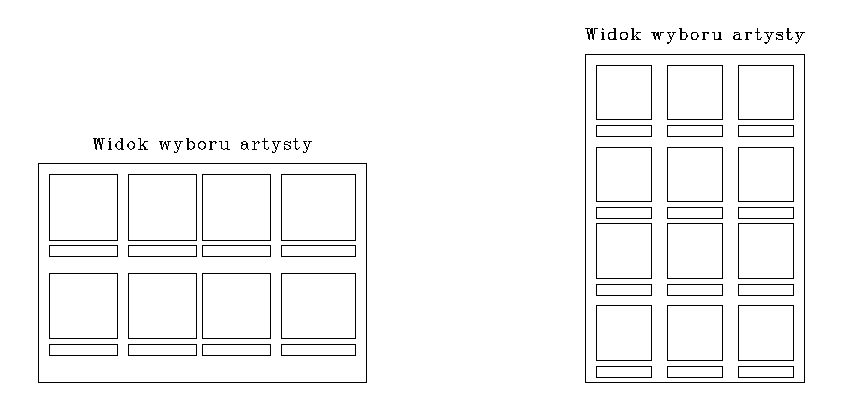
\includegraphics[width=1\linewidth]{images/mockup2_artysta}
	\caption{\centering{Mockup widoku biblioteki - listing wykonawców}}
	\label{fig:mockup2artysta}
\end{figure}

Widok wykonawców, jest przedstawiony na rysunku nr.~\ref{fig:mockup2artysta}. Ten widok będzie ekranem startowym aplikacji. Jako "Kafelki", zwracać będzie się dokument do ułożonych równomiernie na rysunku kwadratów. Na każdym z nich napisana będzie nazwa danego wykonawcy. Klikanie na jeden z nich przejdzie do widoku albumów danego wykonawcy.

\begin{figure}[H]
	\centering
	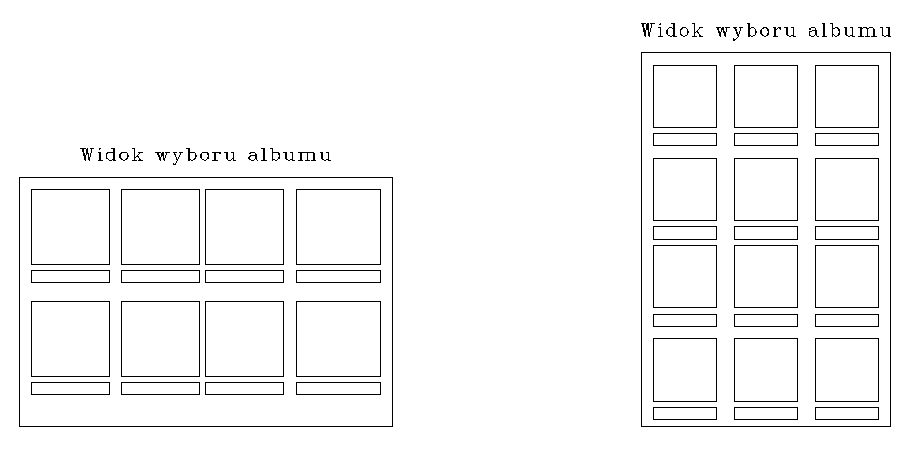
\includegraphics[width=1\linewidth]{images/mockup2_albumy}
	\caption{\centering{Mockup widoku albumów danego wykonawcy}}
	\label{fig:mockup2albumy}
\end{figure}

Widok albumów jest przedstawiony na rysunku nr.~\ref{fig:mockup2albumy}. Widok będzie podobny do widoku wykonawców. Różni się on tym, że na "kafelkach", będą pokazane zdjęcia poszczególnych albumów. Pod "kafelkami", znajdują się nazwy danych albumów.

\begin{figure}[H]
	\centering
	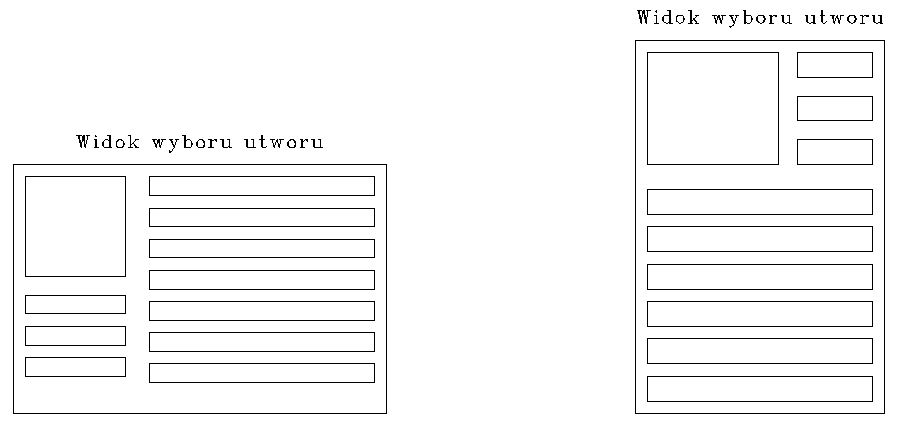
\includegraphics[width=1\linewidth]{images/mockup2_utwory}
	\caption{\centering{Mockup widoku wyboru utworu}}
	\label{fig:mockup2utwory}
\end{figure}


Rysunek nr.~\ref{fig:mockup2utwory} przedstawia ekran pokazujący się po wybraniu albumu. Po wejściu na jakiś album zaprezentowane zostaną zawarte w nim utwory. W lewym górnym kwadrat to zdjęcie danego albumu, a obok niego jest kilka informacji o albumie jak wykonawca, data, tytuł, w postaci tekstu. Dłuższe paski zawarte na dole to lista piosenek, w postaci przycisków z napisanymi, tytułami które można kliknąć, aby daną piosenkę włączyć.

\begin{figure}[H]
	\centering
	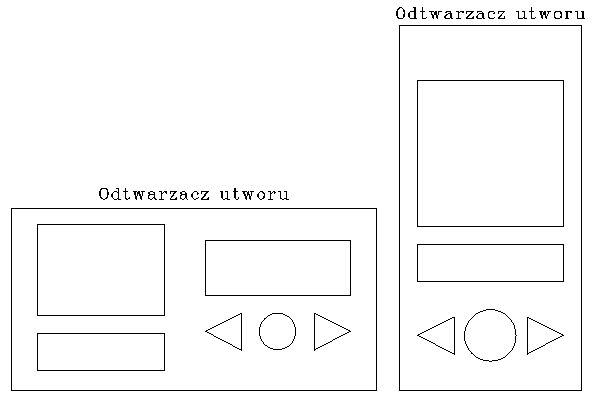
\includegraphics[width=1\linewidth]{images/mockup3_odtwarzacz}
	\caption{\centering{Mockup widoku wyboru utworu}}
	\label{fig:mockup3odtwarzacz}
\end{figure}

Wygląd interfejsu odtwarzacza został zaprezentowany na rysunku nr.\ref{fig:mockup3odtwarzacz}. W widoku horyzontalnym po lewej stronie na górze znajduje się obraz albumu a na dole pod obrazem będzie nazwa utworu, po prawej stronie na górze znajduje się pasek przewijania w formie soundwave któy jest wyciągany z pliku muzycznego a na dole pod soundwave znajdują się przyciski pozwalające na manipulację utworem jak np. na zatrzymanie go lub przewinięcie. W widoku horyzontalnym na samym dole znajduje się zdjęcie albumu, poniżej nazwa utworu, potem soundwave a na końcu przyciski manipulacyjne.

   \newpage
\section{Określenie wymagań szczegółowych}		%2
%Dokładne określenie wymagań aplikacji (cel, zakres, dane wejściowe) – np. opisać przyciski, czujniki, wygląd layautu, wyświetlenie okienek. Opisać zachowanie aplikacji – co po kliknięciu, zdarzenia automatyczne. Opisać możliwość dalszego rozwoju oprogramowania. Opisać zachowania aplikacji w niepożądanych sytuacjach.

\subsection{Ogólny opis wymagań projektu}

Aplikacja jest zaprojektowana w Android Studio w języku Kotlin. Całe UI aplikacji będzie zbudowane na podstawie Frameworka Jetpack Compose\cite{doc_compose} Używając wbudowanych bibliotek w SDK Androida, będzie mogła odczytywać pliki ze wskazanego folderu. Odczytywanie tagów z plików odbędzie się za pomocą biblioteki Taglib\cite{doc_ktaglib}, która posiada nieoficjalne bindingi do Kotlina. Wszelki processing audio np. na potrzeby wizualizacji może zostać wykonany za pomocą SDK i wbudowanego modułu AudioProcessor\cite{doc_audioproc}. Odtwarzaniem pliku będzie się zajmował moduł MediaPlayer\cite{doc_mediaplayer}.

\subsection{Ogólny zarys narzędzi użytych w projekcie}

\subsubsection{Android Studio}

Android Studio jest IDE stworzonym przez Google, na bazie InteliJ IDEA od JetBrains. Jest ono przystosowane, jak z nazwy wynika, do tworzenia aplikacji na Androida. Ku temu celu posiada wiele udogodnień, odróżniających program od typowego edytora jak np. wbudowany emulator Androida, integrujący się z całym środowiskiem, czy preview różnych elementów interfejsu - gdzie elementy te generowane są w kodzie, a nie w osobnym języku jak np. xml - bez potrzeby dekompilacji całej aplikacji. 

Android Studio został użyty w projekcie, ponieważ:

\begin{itemize}
	\item Sam program jest crossplatformowy - nasz zespół używa wielu systemów operacyjnych. Platformy takie jak \texttt{MAUI}, są zespolone z Visual Stdio, czyli z Windowsem. Android Studio jest dostępny na wszystkie większe systemy operacyjne, co ułatwia nam pracę.
	\item Jest to program, zbudowany na podstawie IdeaJ, czyli zagłębiony jest w tym ekosystemie. Oznacza to dostęp do większej ilości pluginów niż np. Visual Studio, nie wspominając o ogólnej możliwości dostosowania ustawień.
\end{itemize}

Wady korzystania z Android Studio to m.in.

\begin{itemize}
	\item Duże wykorzystanie zasobów - program lubi zżerać duże ilości RAMu. W tym momencie, mając otwarty mały projekt + emulator, program wykorzystuje ponad 9GB RAMu. 
\end{itemize}

\subsubsection{Kotlin}

Kotlin został stworzony w 2010 roku przez firmę JetBrains oraz jest on przez nią rozwijany. Kotlin jest wieloplatformowym językiem typowanym statystycznie który został zaprojektowany aby współpracować z maszyną wirtualną Javy. Swoją nazwę zawdzięcza wyspie Kotlin która znajduje się w zatoce finlandzkiej.

Kotlin jest wykorzystywany w projekcie ze względów:

\begin{itemize}
	\item Jest on wspierany przez Android Studio, razem z Javą i C++. Kotlin ponadto, ma dostęp do nowoczesnych frameworków jak Jetpack Compose
	
	\item Jest on \textit{defakto} językiem do programowania na Androida - do niedawna Java mogła cieszyć się tym tytułem, ale od 2019 r. Google ogłosiło Kotlina jako rekomendowany język do tworzenia aplikacji na Android.
\end{itemize}

Składnia Kotlina wygląda następująco:

\begin{lstlisting}[caption=kotlin001 - Funkcje, label={lst:listing-k}, language=kotlin]
fun main() {
	printf("Czesc to ja, kotlin!")
}
\end{lstlisting}
Definicja funkcji wykonywana jest za pomocą "fun".

Zmienne w Kotlinie deklarowane są za pomocą \texttt{val} i \texttt{var}. Różnica polega na tym, że zmienne oznaczone \texttt{val} mogą zostać modyfikowane natomiast zmienne oznaczone \texttt{val} już nie.

\begin{lstlisting}[caption=kotlin002 - Zmienne, label={lst:listing-k}, language=kotlin]
	fun main() {
		var nazwa = "Projekt Android"
		val liczba = "777"
	}
\end{lstlisting}

Kompilator Kotlina posiada funkcję autodedukcji typów, więc w wielu wypadkach typu zmiennej nie trzeba adnotować.

\subsection{Wykorzystanie czujników}

\begin{itemize}
	\item Żyroskop - Z racji, że każdy element interfejsu w Jetpack jest generowany kodem, można, przynajmniej na początku, ustawić każdą wersję interfejsu jako osobną funkcję. Następnie, w zależności od wykrytej orientacji, przy użyciu API sensorów\cite{doc_sensorapi}, można wywoływać odpowiednią funkcję.
	
	\item Mikrofon - Funkcja dyktafonu najprawdopodobniej będzie całkiem oddzielnym Activity. Funkcjonalność ta, z natury, jest dosyć oddzielna od reszty aplikacji. Nagrania dyktafonem powinny być zapisywane do osobnego folderu. Można by zintegrować nagrania z resztą aplikacji jako osobnego wykonawcę w widoku biblioteki. Mikrofon będzie nagrywany poprzez moduł MediaRecorder\cite{doc_mediarecorder}

	\item Czujnik światła - Android Studio oferuje możliwość definiowania własnych klas zajmujących się kolorystyką. Oznacza to że można używać różnych obiektów w zależności od warunków. Wykrywanie światła będzie się odbywało używając API sensorów\cite{doc_sensorapi}
\end{itemize}


\subsection{Zachowanie w niepożądanych sytuacjach}

Głównym wyjątkiem, na który może napotkać się aplikacja jest błąd odczytu albo plików, albo tagów z pliku. Kotlin, na szczęście, pozwala na łatwe sprawdzanie wartości null danych zmiennych operatorem \texttt{?}. W odpowiednich fragmentach kodu dotyczących ładowania plików, będzie sprawdzana poprawność danych i najprawdopodobniej pojawi się pop-up po stronie użytkownika, że wystąpił błąd, a po stronie dewelopera błąd zostanie logowany.

\subsection{Dalszy rozwój}

Jeżeli praca nad aplikacją będzie się odbywała w przyszłości, należy skupić uwagę na lepszym zarządzaniu biblioteką (auto tagowanie, pobieranie miniatur z internetu, itp.). Ponadto, należy szukać błędów, które nadal zostały w aplikacji.

   	\newpage
\section{Projektowanie}		%3
%Opis przygotowania narzędzi (git, visual studio). Wybór i opis bibliotek, klas. Szkic layoutów. Pseudo kody. Opisy wykorzystanych algorytmów (np. algorytm sortowania). Dokładniejsze określenie założeń i działania aplikacji, (np.: ten przycisk otworzy takie okno a w tym oknie wpisujemy takie dane).




   	\newpage
\section{Implementacja}		%4
%Wkleić szkielet kodu, wraz z komentarzami. Opisać zmienne, struktury do czego służą. Opisać procedury, metody co wykonują. Opisać nowe zdefiniowane klasy. Opisać dziedziczenie. Opisać nowo utworzone pliki za co odpowiadają.

\subsection{Zarządzanie bazą danych}

\subsubsection{Klasa \texttt{DatabaseManager}} \label{sec:DatabaseManager}

Za zarządzanie bazą danych odpowiedzialna jest klasa \texttt{DatabaseManager}, której kod jest zamieszony na listingu nr. \ref{lst:DatabaseManager_struct}. Klasa jest wrapperem do bazy danych \texttt{Room}\cite{doc_room} i do niej akcesorów.

\begin{lstlisting}[caption=Strukutura klasy \texttt{DatabaseManager}, label={lst:DatabaseManager_struct}, language=kotlin]
@Singleton
class DatabaseManager @Inject constructor(
    @ApplicationContext context: Context
) {
    private val database: LibraryDb = Room.databaseBuilder(
        context,
        LibraryDb::class.java, "Library"
    ).build()

    fun collectAuthorsFlow(): Flow<List<Author>> = database.uiDao().getAllAuthorsFlow()

    fun collectAlbumsByAuthorFlow(authorName: String): Flow<List<Album>> {
        return database.uiDao().getAuthorWithAlbums(authorName)
            .map { it.albums }
    }

    fun collectSongsByAlbumFlow(albumId: Long): Flow<List<Song>> {
        return database.uiDao().getAlbumWithSongs(albumId)
            .map { it.songs }
    }
	
...

    fun populateDatabase(songs: List<TagExtractor.SongInfo>) {
        assert(Thread.currentThread().name != "main")

        val dao = database.logicDao()

        fun addAuthors() {
            songs.fastForEach { song ->
                //TODO: there should be a distinction between albumartists and regular artists
                song.albumArtists?.fastForEach { name ->
                    if(dao.getAuthor(name) == null) {
                        dao.insertAuthor(Author(name = name))
                    }

                }
            }
        }

        fun addAlbumsAndRelations() {
            // FIXME: xdddddddd
            val distinctAlbumArtistsList = songs
                .map { Triple(it.album, it.albumArtists, it.coverUri) }
                .distinct()
            Log.d(javaClass.simpleName, "Distinct artists set: $distinctAlbumArtistsList")

            distinctAlbumArtistsList.fastForEach {
                val albumTitle = it.first.toString()
                val artists = it.second
                val coverUri = it.third

                val albumId = dao.insertAlbum(Album(
                    title = albumTitle,
                    coverUri = coverUri.toString(),
                ))

                artists?.fastForEach {
                    dao.insertAlbumAuthorCrossRef(AlbumAuthorCrossRef(
                        albumId = albumId,
                        name = it.toString()
                    ))
                }
            }
        }

        fun addSongs() {
            songs.fastForEach { song ->
                Log.d(javaClass.simpleName, "NEW SONG\n")
                Log.d(javaClass.simpleName, "Album artists: ${song.albumArtists}")

                val albumWithAuthorCandidates = dao
                    .getAlbumsByTitle(song.album.toString())
                    .map { it.albumId }
                    .map { dao.getAlbumWithAuthors(it) }
                Log.d(javaClass.simpleName, "$albumWithAuthorCandidates")

                var correctAlbum: Album? = null
                albumWithAuthorCandidates.fastForEach {
                    Log.d(javaClass.simpleName, "${song.albumArtists}, ${it.authors}")
                    //FIXME: theese guys shouldn't be ordered, will have to refactor a bunch of
                    // stuff with sets instead of lists
                    if(song.albumArtists?.sorted() == it.authors.map { it.name }.sorted()) {
                        correctAlbum = it.album
                    }
                }

                dao.insertSong(Song(
                    title = song.title,
                    albumId = correctAlbum?.albumId,
                    fileUri = song.fileUri.toString(),
                ))
            }
        }

        addAuthors()
        addAlbumsAndRelations()
        addSongs()
    }
}
\end{lstlisting}

% TODO: opisac co to hilt
Na pierwszej linijce można zauważyć adnotację \texttt{@Singleton}. Pochodzi ona z bilbioteki \texttt{Hilt}\cite{doc_hilt}. Powiadamia ona bibliotekę o tym że klasa jest singletonem, czyli że ma istnieć tylko jej jedna instancja na cały program. Uczyniono to, dlatego że baza danych powinna być jedna na całą aplikację. Menadżer z nią interfejsujący, dlatego że jest używany w wielu innych klasach, też powinien mieć tylko jedną instancję, aby nie marnować pamięci.

Na linijce nr. 2, widać konstruktor klasy, do którego też przy użyciu \texttt{Hilt}, wstrzykiwany jest \texttt{context}.

Następnie, na linijce nr. 5, widać inicjalizację samego obiektu bazy \texttt{database}. Baza jest reprezentowana przez klasę \texttt{LibraryDb}, definicję której można zobaczyć w sekcji \ref{sec:LibraryDb}

% TODO: opisac co to flow albo w 2 chapterze albo 3
Dalej, do linijki nr. 22 pokazane są metody zwracające rózne elementy bazy. Wiekszosc z tych metod zwraca \texttt{Flow}\cite{TODO:}. \texttt{Room} natywnie obsługuje \texttt{Flowy}, a dlatego że wymusza dostęp do bazy z innych wątków niż główny, większość operacji wykonywanych na bazie odbywa się za pośrednictwem typów \texttt{Flow}

Same metody są wrapperami do obiektów \texttt{Dao} bazy. Więcej o nich w sekcji \ref{sec:daos}. Niektóre obrabiają dane jak np. \texttt{collectSongsByAlbumFlow()} na linijce nr. 17., która mapuje zwraca piosenki z wyjściowej klasy relacyjnej.

Metod tych jest więcej, lecz wyglądają one bardzo podobnie. Dla zwięzłości, mozna je pominąć.

%TODO: TagExtractor.SongInfo to będzie po prostu SongInfo jak sie mi zeche w kodzie zmienic
Metoda \texttt{populateDatabase()} zadeklarowana na linijce nr. 24, jest odpowiedzialna za ładowanie wyjętych z plików informacji do bazy. Jako parametr odstaje ona zmienną \texttt{songs} typu \texttt{List<TagExtractor.SongInfo>}   Zadeklarowane są w niej trzy funkcje pomocnicze: \texttt{addAuthors()}, \texttt{addAlbumsAndRelations()} i \texttt{addSongs()}. Wywoływane są one po kolei w metodzie głównej.

Funkcja \texttt{addAuthors()}, zadeklarowana na linijce nr. 29, jest prosta w swoim działaniu. Lista z \texttt{SongInfo} jest iterowana i po kolei wpisywani są wszyscy autorzy, którzy jeszcze w bazie nie istnieją.

Funkcja \texttt{addAlbumsAndRelations()}, zadeklarowana na linijce nr. 41, odpowiada za dodawanie albumów do bazy oraz tworzenie relacji między nimi, a autorami. Tworzona zmienna \texttt{distinctAlbumArtistsList} mapuje tylko unikalne pary albumów i autorów (zmienna \texttt{coverUri} nie ma znaczenia przy określaniu autorstwa, jest przypisywana tutaj dlatego, że trudno było znaleźć dla niej lepsze miejsce). Dzięki temu początkowemu filtrowaniu, wiadomo, że każdy napotkany album będzie unikalny. Następnie, \texttt{distinctAlbumArtistsList} jest iterowana - przy każdej iteracji dodawany jest nowy album do bazy. Metoda \texttt{insertAlbum()} zwraca \texttt{id} nowo dodanego albumu. Wynik jej jest przypisywany do zmiennej \texttt{albumId} na linijce nr. 53. Potem, zostaje przypisywana relacja albumu z autorami. Autorów może być kilku, więc są oni reprezentowani przy każdej iteracji przez listę, która jest iterowana, a relacja zostaje dodawana z nazwą autora i \texttt{albumId}.

Funkcja \texttt{addSongs()}, zadeklarowana na linijce nr. 67, ma na celu dodanie piosenek do bazy. Ciało funkcji jest w pętli iterującej się przez listę piosenek. Na początku pętli, na linijce nr. 72 deklarowana jest zmienna \texttt{albumWithAuthorCandidates}. Jest ona listą relacji album - autorzy wszystkich albumów o tej samej nazwie co ten w danym elemencie listy. Następnie, lista ta jest iterowana i przy każdej iteracji sprawdzane jest czy lista autorów w danej relacji jest równa z listą autorów danej piosenki. Jeżeli tak, wartość danego albumu z wybranej relacji jest przypisywana do zmiennej zadeklarowanej na lini nr. 78 \texttt{correctAlbum}. Na końcu funkcji, piosenka dodana jest do bazy przy użyciu metody \texttt{dao}.

\subsubsection{Klasa LibraryDb} \label{sec:LibraryDb}

Klasa \texttt{LibraryDb} jest deklaracją faktycznej instancji bazy danych, która jest implementowana i generowana przez bibliotekę \texttt{Room}. Z racji tego, że jest to klasa abstrakcyjna, jej zadaniem jest określenie struktury bazy i jakie komponenty ma ona zawierać

\begin{lstlisting}[caption=Deklaracja bazy LibraryDb, label={lst:LibraryDb_class}, language=kotlin]
@Database(entities = [Song::class, Author::class, Album::class, AlbumAuthorCrossRef::class], version
= 1)
abstract class LibraryDb : RoomDatabase() {
    abstract fun logicDao(): LogicDao
    abstract fun uiDao(): UIDao
}

\end{lstlisting}

Jak widać na listingu nr.~\ref{lst:LibraryDb_class}, na początku klasy należy zamieścić adnotację \texttt{@Database}. Powiadamia ona bibliotekę \texttt{Room} o tym, że następująca klasa jest bazą danych. Parametr \texttt{entities} określa wszystkie tabele jakie mają się w klasie zawierać. O tabelach więcej w sekcji nr.~\ref{sec:tables}. Parametr \texttt{version} zajmuje się wersjonowaniem bazy. Jest on ważny przy aktualizacjach aplikacji, aby baza mogła zostać odpowiednio zmieniona. 

Na linijce nr. 3 umieszczona jest faktyczna deklaracja klasy. Dziedziczy ona z klasy \texttt{RoomDatabase}. Jedyne rzeczy jakie są do dziecięcej klasy dodawane, to metody zwracające obiekty \texttt{dao}, opisane w sekcji nr.~\ref{sec:daos}.

%TODO: 
\subsubsection{Obiekty Dao} \label{sec:daos}

\subsubsection{Tabele} \label{sec:tables}

W bibliotece \texttt{Room}, każda tabela to \texttt{dataclass} określana adnotacją \texttt{@Entity}. Kolumny takiej tabeli to po prostu pola klasy. Klucz danej tabeli jest określany adnotacją \texttt{@PrimaryKey}

\paragraph{Author}

\begin{lstlisting}[caption=Deklaracja tabeli Author, label={lst:Author_class}, language=kotlin]
@Entity
data class Author (
    @PrimaryKey val name: String
)
\end{lstlisting}

Tabela \texttt{Author}, zawarta na listingu nr.~\ref{lst:Author_class}, określa autorów. Tabela jest prosta, jedynym polem jest \texttt{name}, który jest kluczem.

\paragraph{Album}

\begin{lstlisting}[caption=Deklaracja tabeli Album, label={lst:Album_class}, language=kotlin]
@Entity
data class Album(
    @PrimaryKey(autoGenerate = true) val albumId: Long = 0,
    val title: String,
    val coverUri: String?,
)
\end{lstlisting}

Tabela \texttt{Album}, zawarta na listingu nr.~\ref{lst:Album_class}, określa albumy. Kluczem jest zmienna \texttt{albumId}. Klucz jest generowany automatycznie, dzięki parametrowi adnotacji \texttt{autoGenerate}. Pole \texttt{title} określa tytuł, a pole \texttt{coverUri} określa adres \texttt{URI} okładki.

\paragraph{Song}

\begin{lstlisting}[caption=Deklaracja tabeli Song, label={lst:Song_class}, language=kotlin]

@Entity(
    foreignKeys = [
        ForeignKey(
            entity = Album::class,
            parentColumns = ["albumId"],
            childColumns = ["albumId"],
            onDelete = ForeignKey.CASCADE
        )
    ],

    indices = [Index(value = ["albumId"])]
)
data class Song(
    @PrimaryKey(autoGenerate = true) val songId: Long = 0,
    val title: String?,
    val albumId: Long?,
    val fileUri: String?,
)

\end{lstlisting}

Klasa ta, zawarta na listingu nr.~\ref{lst:Song_class}, określa tabelę piosenek. Pole \texttt{foreignKeys} w adnotacji \texttt{@Entity} określa obce klucze, którymi posługuje się klasa (więcej o tym w sekcji nr.~\ref{sec:relations}). Pole \texttt{indices} każe indeksować pola z \texttt{albumId} ku polepszeniu szybkości bazy. W ciele klasy, pole \texttt{title} to tytuł piosenki. Pole \texttt{albumId} określa ID albumu, do którego należy dana piosenka. 

\subsubsection{Relacje} \label{sec:relations}

   	\newpage
\section{Testowanie}	%5
%Opisujemy testy, sprawdzamy czy nie generuje błędów.

\subsection{Włączenie aplikacji}
\newpage

\begin{figure}[H]
	\centering
	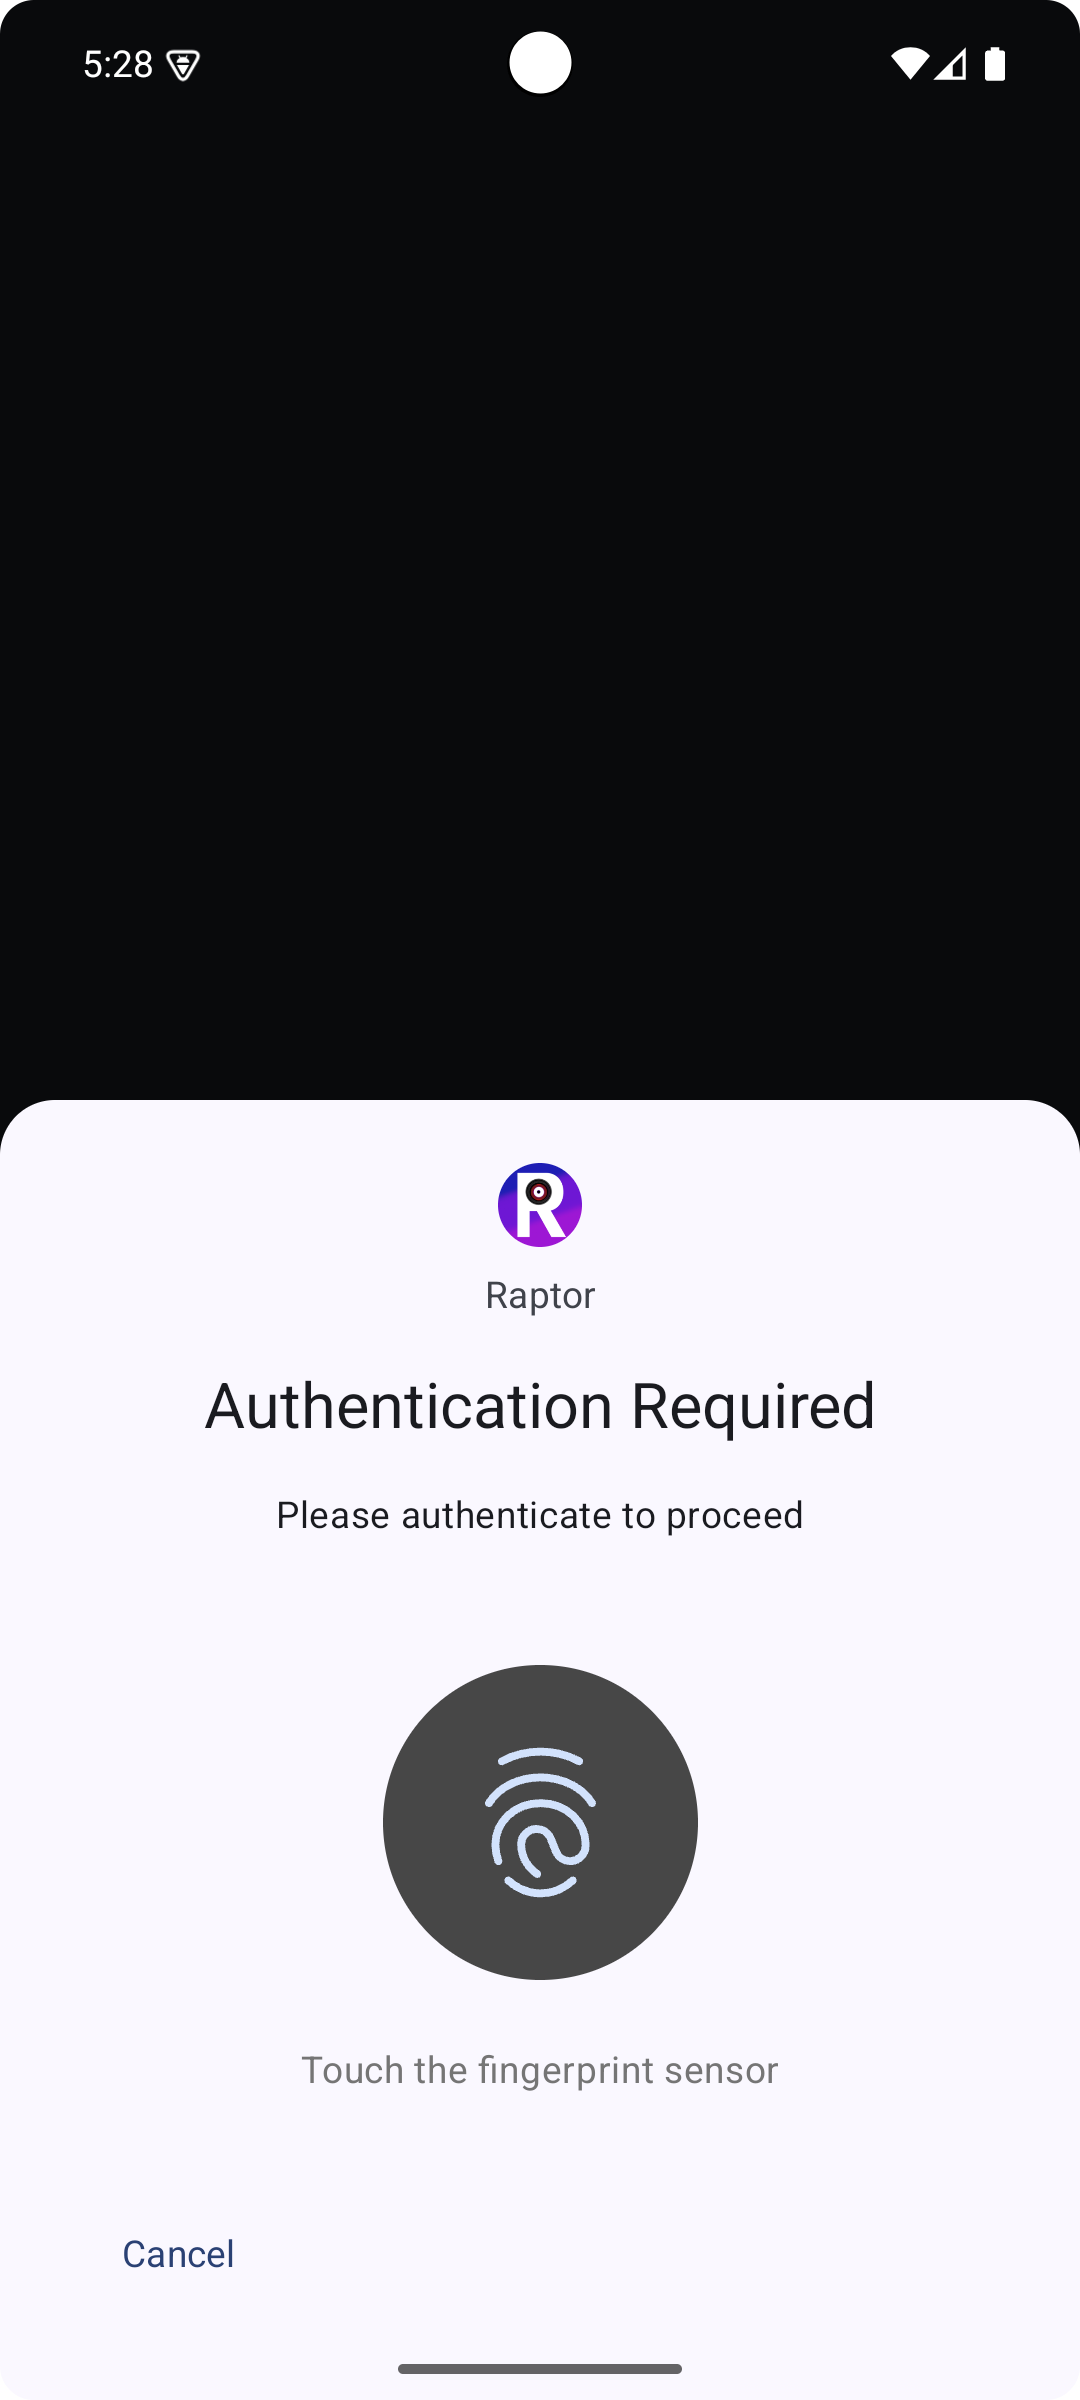
\includegraphics[width=1\textwidth]{images/usage_fingerprint.png}
	\caption{\centering{Prośba o podanie odcisku palca.}}
	\label{fig:test_fingerprint}
\end{figure}

\begin{figure}[H]
	\centering
	
\includegraphics[width=1\textwidth]{images/tutorial_autorzy_pusty.png}
	\caption{\centering{Widok po zweryfikowaniu odcisku.}}
	\label{fig:test_autorzy_pusty}
\end{figure}

Zgodnie z założeniami, po otwarciu aplikacji pojawia się prośba o podanie odcisku palca (rysunek nr.~\ref{fig:test_fingerprint}). Po zweryfikowaniu, aplikacja pomyślnie przechodzi do głównego ekranu, jak pokazano na rysunku nr.~\ref{fig:test_autorzy_pusty}.

\subsection{Dodawanie utworów}

\begin{figure}[H]
	\centering
	
\includegraphics[width=1\textwidth]{images/tutorial_select_folder.png}
	\caption{\centering{Włączenie wyboru folderu.}}
	\label{fig:test_select_folder}
\end{figure}

\begin{figure}[H]
	\centering
	
\includegraphics[width=1\textwidth]{images/tutorial_folder_selected.png}
	\caption{\centering{Wybieranie folderu z muzyką.}}
	\label{fig:test_folder_selected}
\end{figure}

\begin{figure}[H]
	\centering
	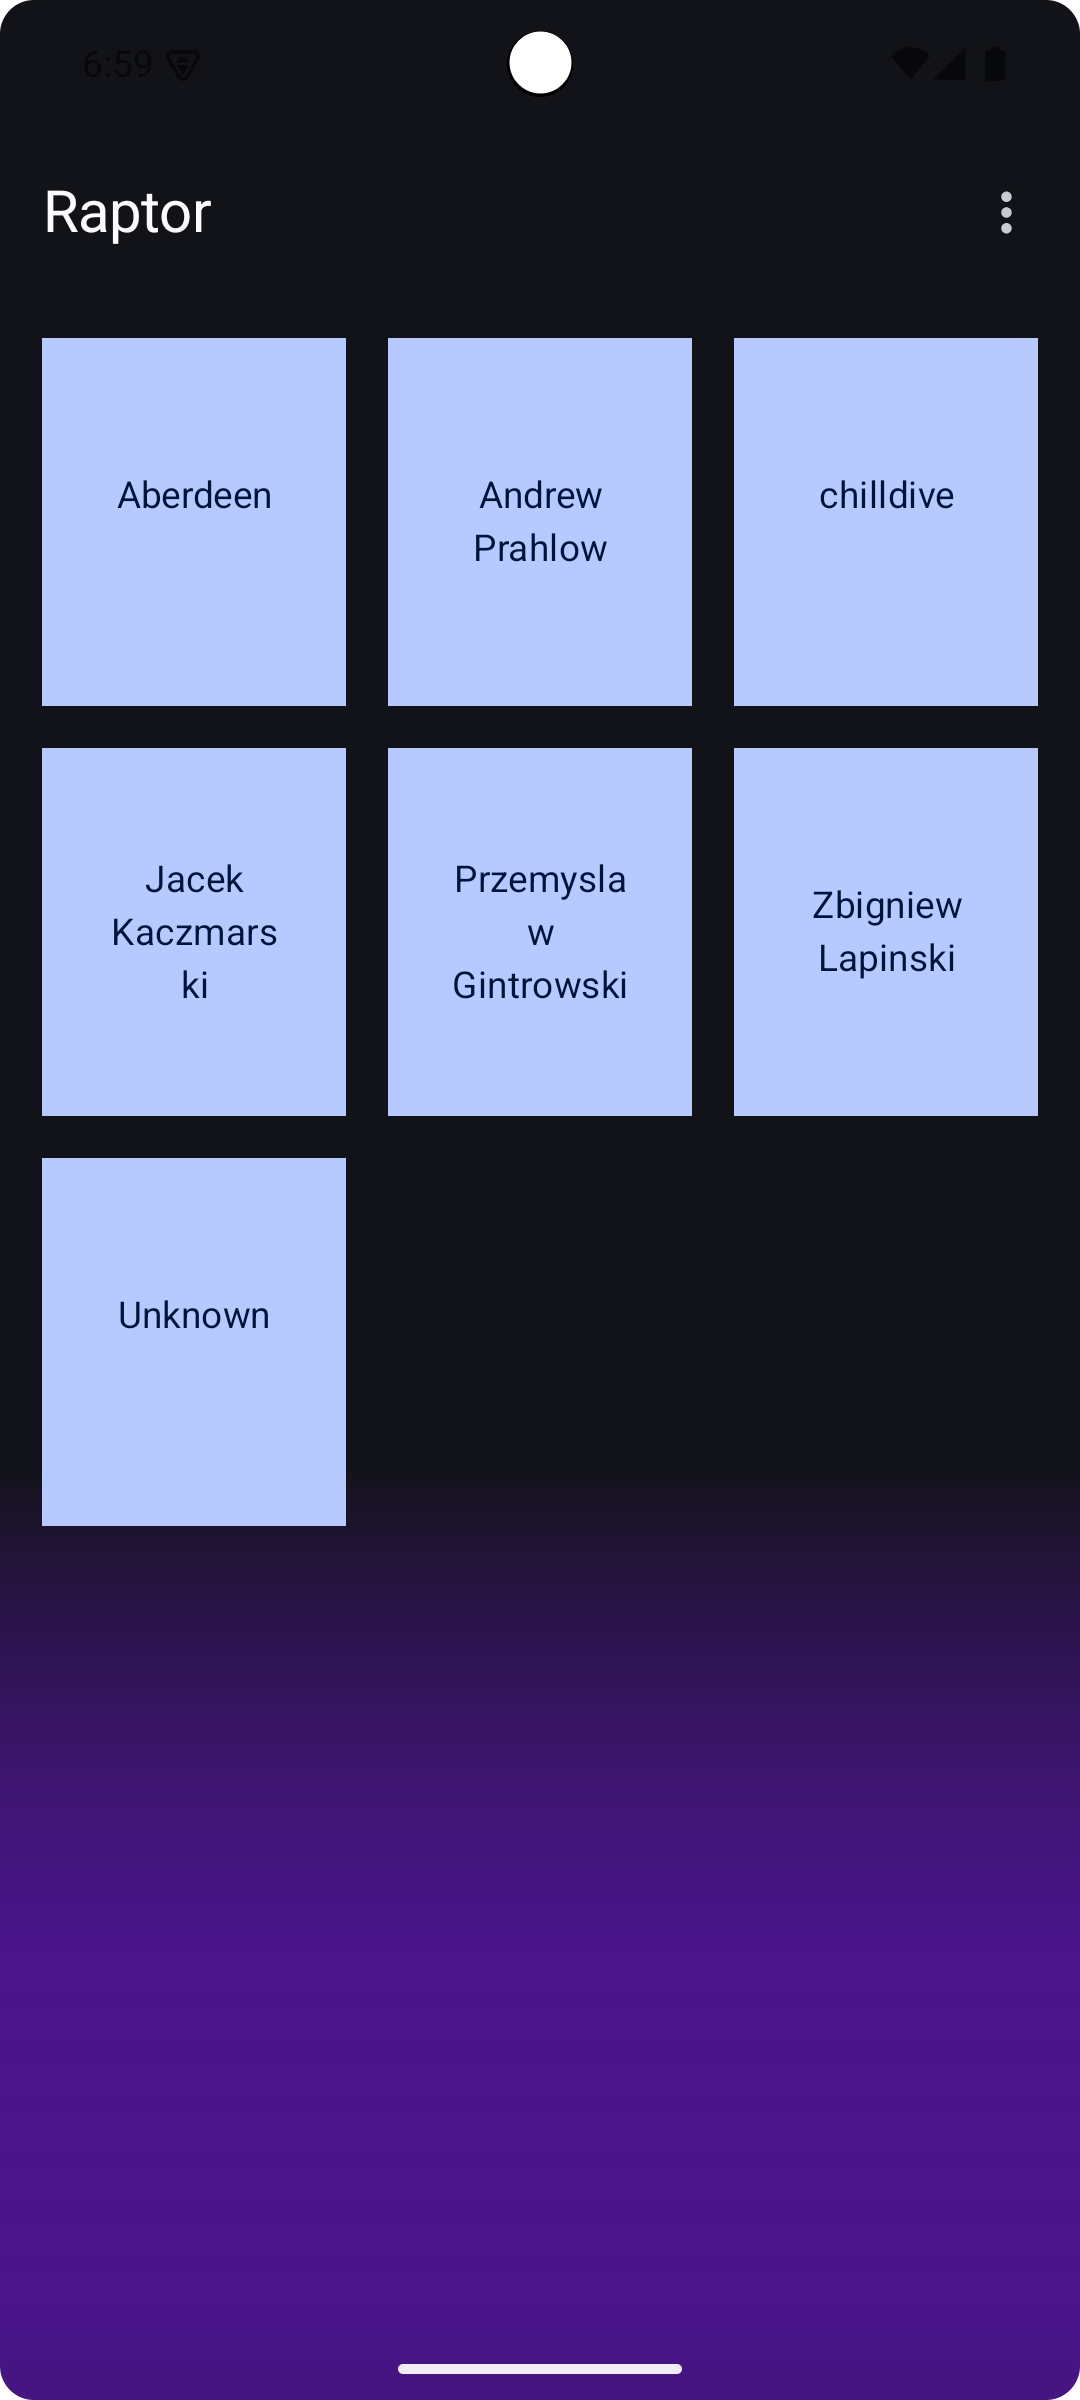
\includegraphics[width=1\textwidth]{images/tutorial_after_loading.png}
	\caption{\centering{Widok po załadowaniu plików.}}
	\label{fig:test_after_loading}
\end{figure}

Na rysunkach nr. \ref{fig:test_select_folder}, \ref{fig:test_folder_selected} i \ref{fig:test_after_loading} ukazana jest procedura ładowania plików piosenek. Jak widać piosenki załadowały się pomyślnie i interfejs odpowiednio reaguje na te zmiany. W kafelku o nawie \enquote{Unknown}, zawarte są piosenki bez otagowanego wykonawcy.

\subsection{Nawigacja}

\begin{figure}[H]
	\centering
	
\includegraphics[width=1\textwidth]{images/tutorial_album_view.png}
	\caption{\centering{Widok po wejściu w autora.}}
	\label{fig:test_album_view}
\end{figure}

\begin{figure}[H]
	\centering
	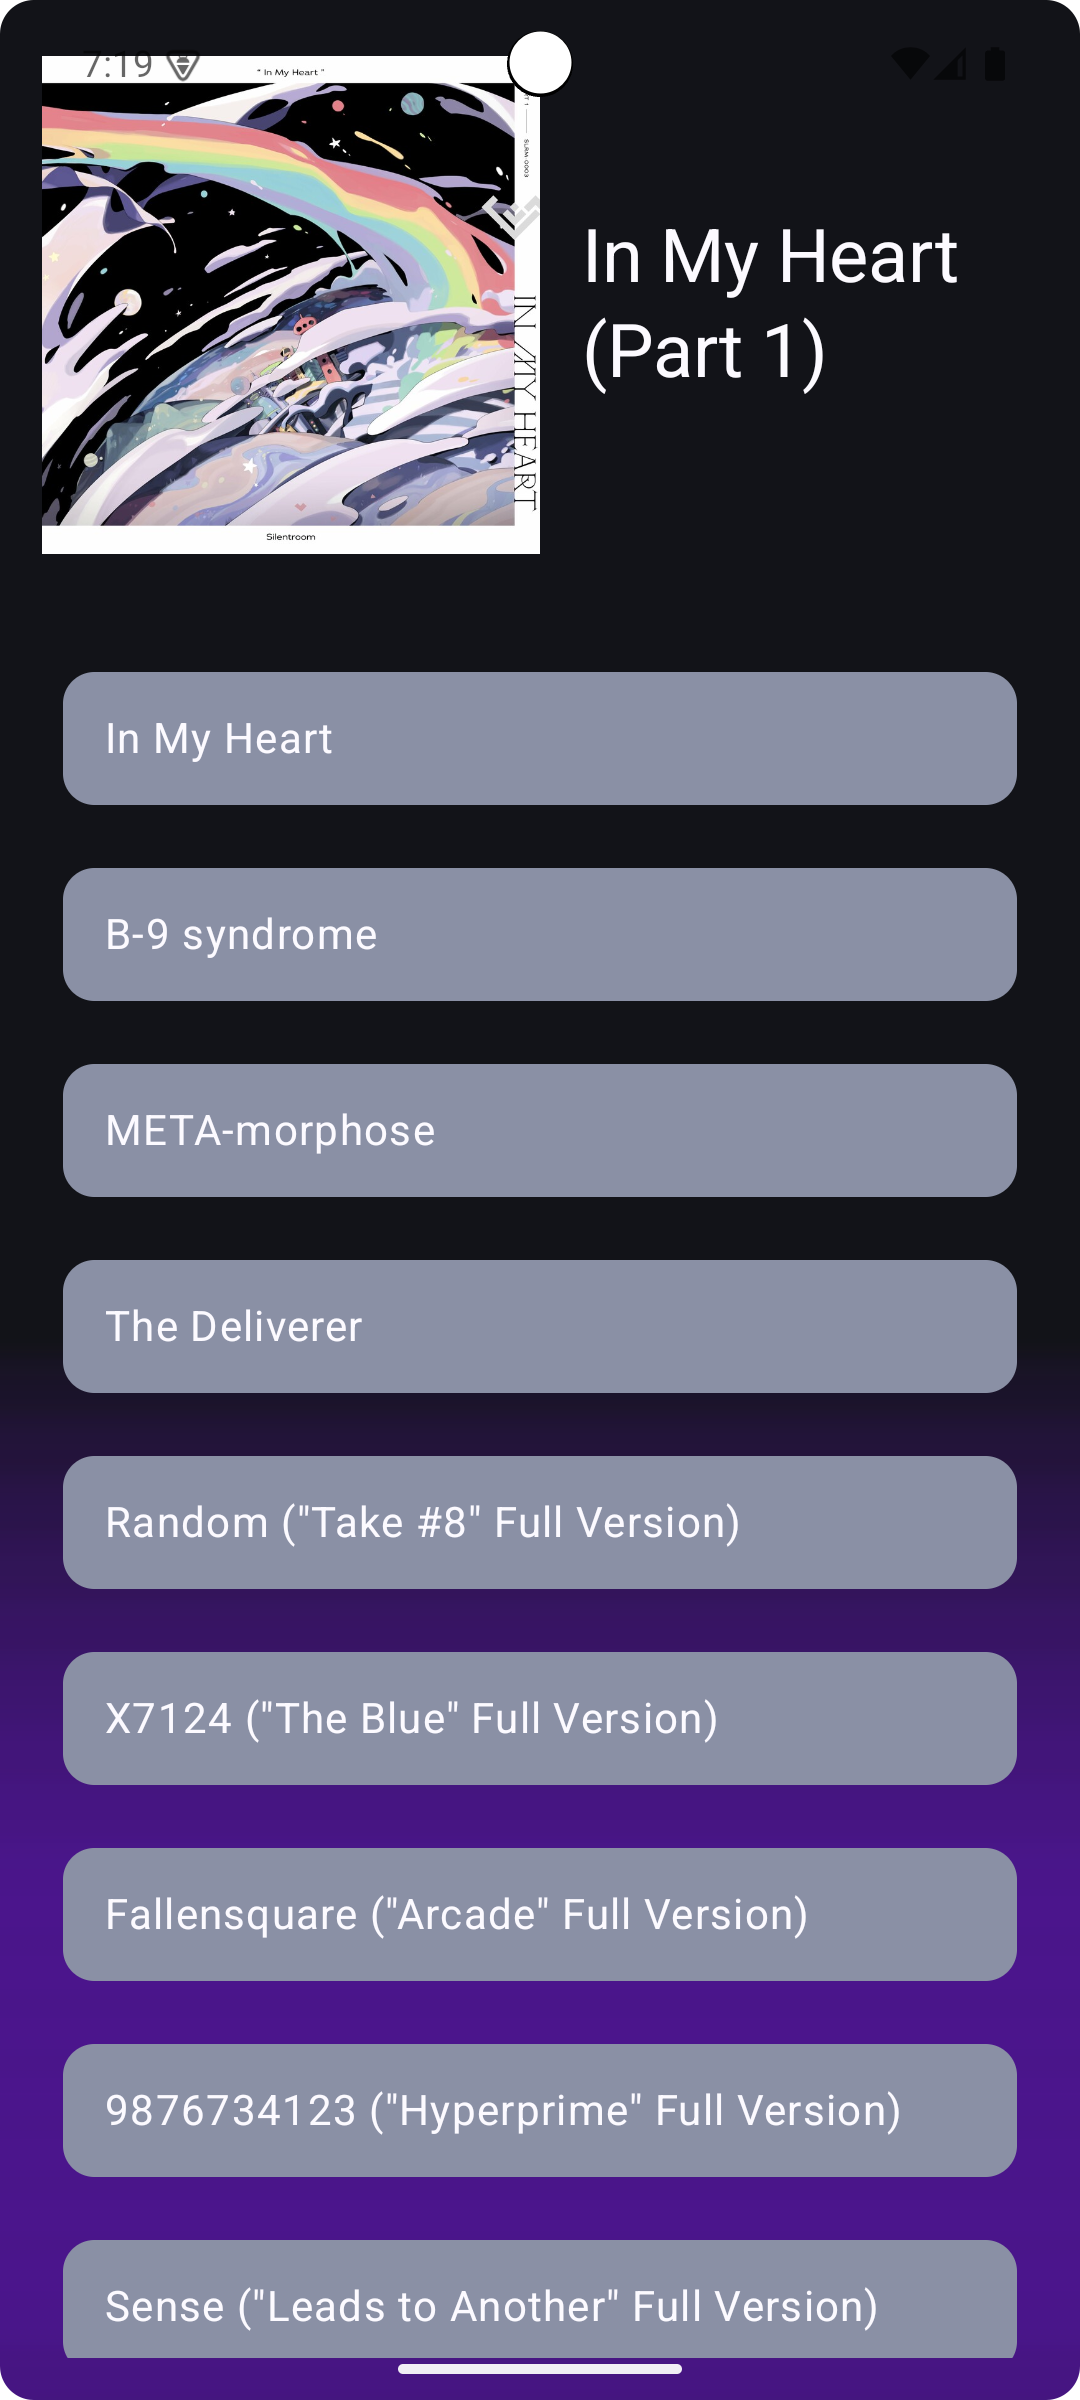
\includegraphics[width=1\textwidth]{images/tutorial_song_view.png}
	\caption{\centering{Widok wyboru piosenki.}}
	\label{fig:test_song_view}
\end{figure}

Na rysunku nr.~\ref{fig:test_album_view} pokazano, że pomyślnie można przejść do ekranu widoku albumów. Pomyślnie wyświetlają się wszystkie miniaturki. Analogicznie, z rys. nr.~\ref{fig:test_song_view} wynika, że można przejść do widoku piosenek. Podobnie, informacje o albumie, w którym są piosenki wyświetlają się pomyślnie. 

\subsection{Działanie odtwarzacza}

\begin{figure}[H]
	\centering
	
\includegraphics[width=1\textwidth]{images/test_player_playing.png}
	\caption{\centering{Odtwarzacz odgrywa piosenkę.}}
	\label{fig:test_player_playing}
\end{figure}

\begin{figure}[H]
	\centering
	
\includegraphics[width=1\textwidth]{images/test_player_paused.png}
	\caption{\centering{Piosenka w odtwarzaczu jest zapauzowana.}}
	\label{fig:test_player_paused}
\end{figure}

\begin{figure}[H]
	\centering
	
\includegraphics[width=1\textwidth]{images/test_player_stopped.png}
	\caption{\centering{Zatrzymany odtwarzacz}}
	\label{fig:test_player_stopped}
\end{figure}

Jak widać na rysunku nr.~\ref{fig:test_player_playing}, odtwarzacz pomyślnie odgrywa piosenkę. Z wiadomych przyczyn, trudno jest pokazać to, że słychać dźwięk. Ponadto pokazana jest miniaturka, generowany jest waverform oraz wyświetlane są informacje o piosence, mianowicie tytuł oraz wykonawcy. Na rysunku nr.~\ref{fig:test_player_paused}, pokazano, że odtwarzacz może być zapauzowany. Przeciągając progress bar do końca, można zauważyć, że pojawia się możliwość zrestartowania utworu.

\begin{figure}[H]
	\centering
	
\includegraphics[width=1\textwidth]{images/test_player_nextcap.png}
	\caption{\centering{Przechodzenie przez album do końca}}
	\label{fig:test_player_nextcap}
\end{figure}

Na rysunku nr.~\ref{fig:test_player_nextcap} pokazano możliwość przechodzenia przez piosenki w albumie, przyciskami obok głównego, na środku. Jak widać na tym samym rysunku program wykrywa, gdy użytkownik dostanie się do ostatniego utworu - zostaje wtedy powiadomiony, że nie może przejść dalej.

   	\newpage
\section{Podręcznik użytkownika}  %6
%Opis jak używać programu. Mogą być z zrzut ekranu razem z opisem. 



       
%%%%%%%%%%%%%%%%%%% koniec treść główna dokumentu %%%%%%%%%%%%%%%%%%%%%
	\newpage
    \addcontentsline{toc}{section}{Literatura}  
	\printbibliography

    \newpage
    \hypersetup{linkcolor=black}
    \renewcommand{\cftparskip}{3pt}
    \clearpage
    \renewcommand{\cftloftitlefont}{\Large\bfseries\sffamily}
    \listoffigures
    \addcontentsline{toc}{section}{Spis rysunków}
	\thispagestyle{fancy}
	
    \newpage
    \renewcommand{\cftlottitlefont}{\Large\bfseries\sffamily}
    \def\listtablename{Spis tabel}
    \addcontentsline{toc}{section}{Spis tabel}\listoftables 
	\thispagestyle{fancy}
	
	\newpage
	\renewcommand{\cftlottitlefont}{\Large\bfseries\sffamily}
	\renewcommand\lstlistlistingname{Spis listingów}
	\addcontentsline{toc}{section}{Spis listingów}\lstlistoflistings 
	\thispagestyle{fancy}
	


    %lista rzeczy do zrobienia: wypisuje na koñcu dokumentu, patrz: pakiet todo.sty
    \todos
    %koniec listy rzeczy do zrobienia
\end{document}
